\section{Genetics}\label{sec:genetics}

\subsection{Definitions}\label{subsec:definitions}

First, it is important to describe what the genetic approach means.
Genetic approach was first introduced by~\cite{hollandAdaptationNaturalArtificial1975} in 1975
to solve optimization problems where it is computationally infeasible to
find an optimal solution by enumerating all possible solutions.

This approach is inspired by nature and Darwin’s Theory of Evolution~\cite{TODO}
– a population of individuals evolving over time.
Individuals that are more adapted to the environment are
more likely to survive and thus pass their genes to the next population.
Thus, over time, population should converge to the state where the adaptation to the environment is the highest.

Holland defines several structures that reassemble this natural process.
The most important ones are described below.\\

\navesti{Allele} represents a concrete value that a gene can have.
It can be thus described as a set of alternatives to choose from. \\

\navesti{Gene} is a structure composed of alleles.
It often describes one trait or characteristic. \\

\navesti{Chromosome} is a structure composed of genes.
Thus it is an amalgam of characteristics described by genes.\\

\navesti{Individual} represents a solution to the problem and is defined by its chromosome.
A numeric value called \textit{fitness} can be assigned to each individual that represents how well the individual performs in an environment. \\

\navesti{Population} is a set of individuals.
It can be interpreted as a subset of possible solutions.\\

One concrete example of the definitions mentioned above is in figure~\ref{fig:population}.
There are two individuals in the population, with their chromosome having two genes.
The first gene is a vector with alleles having values 1 to 5. The second gene is a string vector
with alleles having values $H$ or $V$. Lastly, each individual has a fitness value.
Thus, because A’s fitness $30.5$ is greater than B’s fitness $9.8$, we can say
that individual A performs better than B.


\begin{figure}
    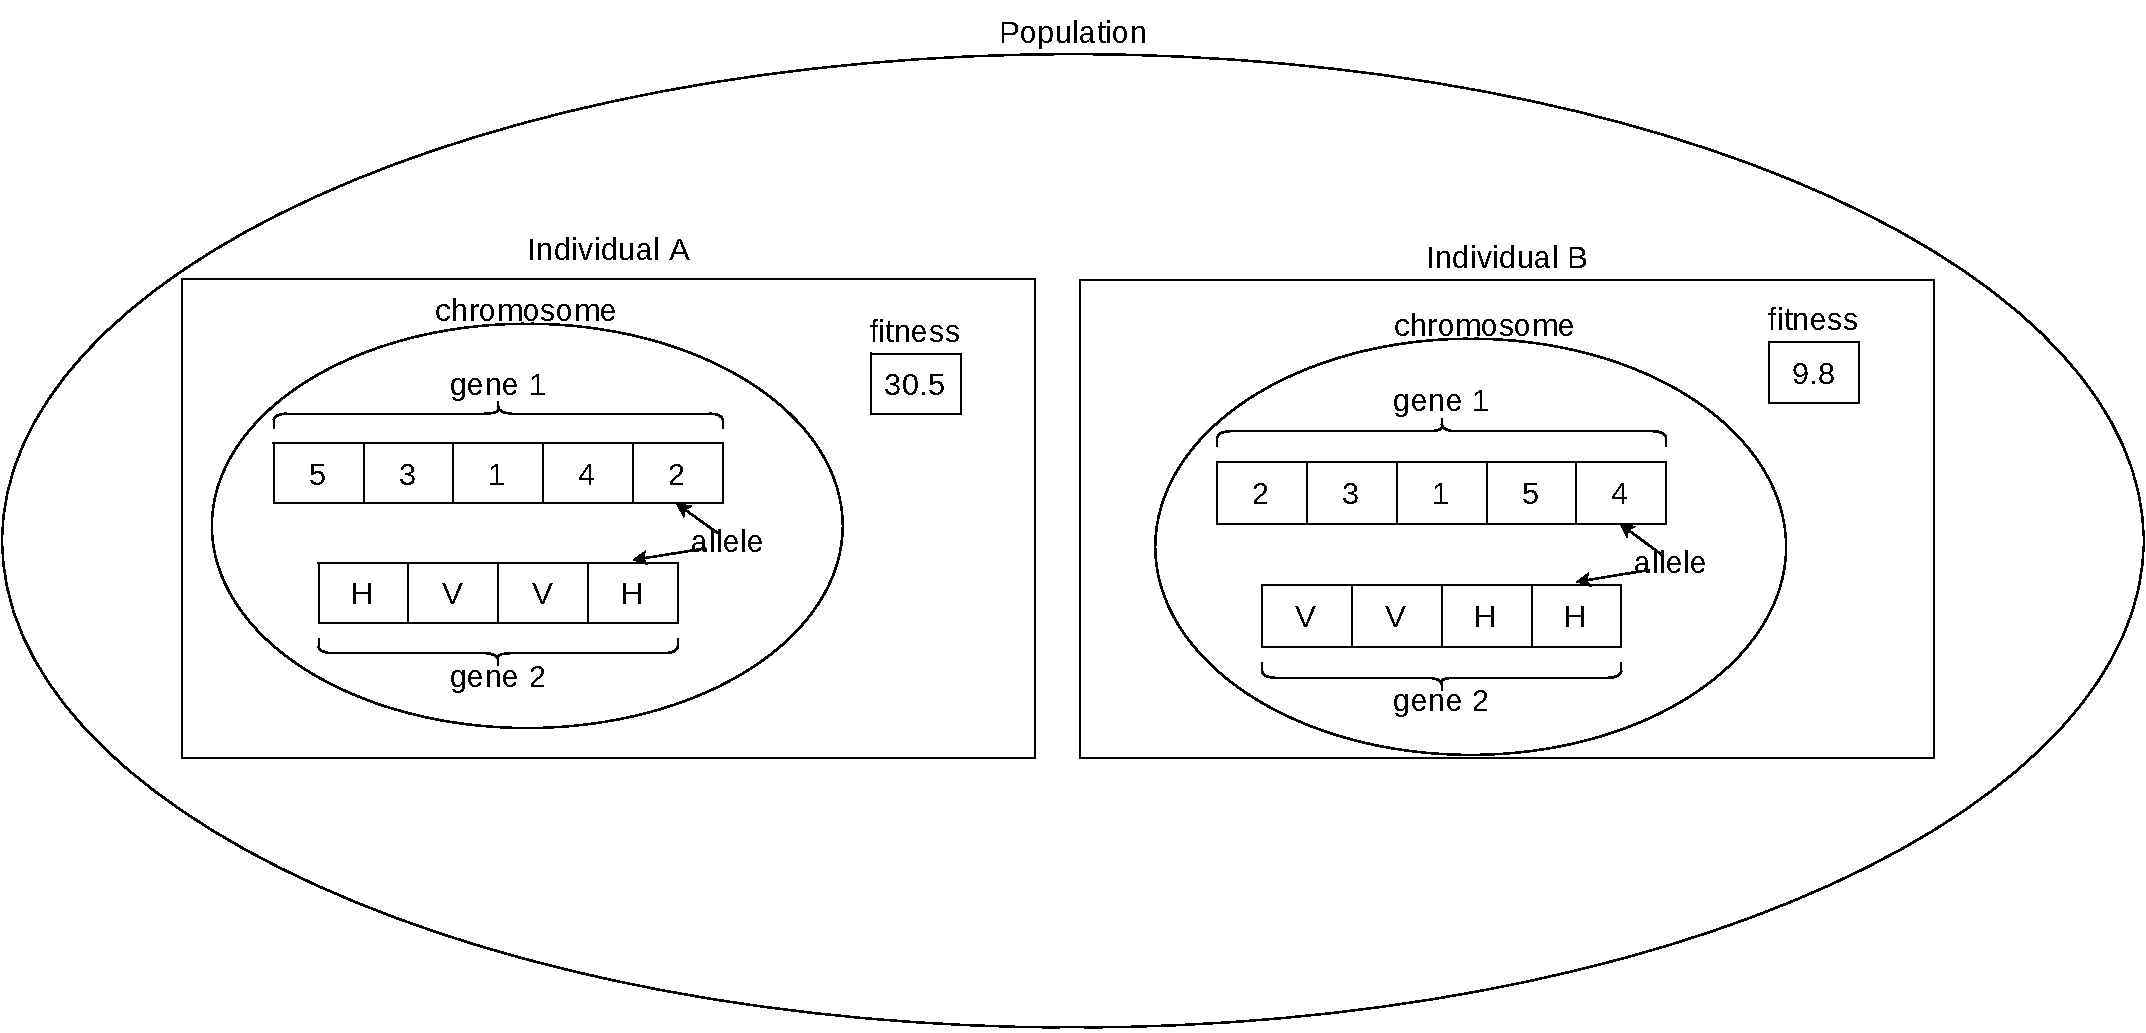
\includegraphics[width=1\textwidth, left]{population}
    \caption[Population example]{Example of a population composed of two individuals.}
    \label{fig:population}
\end{figure}

For the structures defined above, multiple operations called \textit{genetic operators}
were defined by Holland and other researchers following his work.
Two of them that are used in this thesis are described below.\\

\navesti{Crossover} genetic operator takes two individuals as input and, by recombination
of their alleles in their genes, produces a new individual/s called \textit{offspring} or \textit{child}.\\

\navesti{Mutation} genetic operator takes one individual as input and produces a new one
which may have some of its alleles replaced by different random ones.\\

Finally, there needs to be a process that transforms a population
to a new one with the goal of if this transformation process is applied sufficient
number of times to some initial population,
(sub)-optimal solution to the problem will be found.
This process is called \textit{reproductive plan}.\\

\navesti{Reproductive plan} is a process that takes a population on input and produces a modified
population using genetic operators.\\

One example of a reproductive plan is in figure~\ref{fig:reproductive-plan}.
At the start, an initial population of individuals is generated.
Then, for each individual, the fitness value is calculated.
Lastly, genetic operators are applied to produce the new population.
In this example, crossover and mutation.
The process ends if the stopping condition is met.

\begin{figure}[h]
    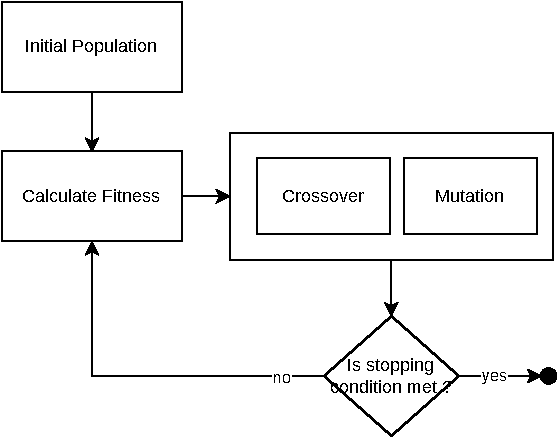
\includegraphics[width=0.65\textheight, center]{reproductive_plan}
    \caption[Example of a reproductive plan]{Example of a reproductive plan with crossover and mutation genetic operators.}
    \label{fig:reproductive-plan}
\end{figure}

\subsection{Schema Theorem}\label{subsec:schema-theorem}

Holland in~\cite{hollandAdaptationNaturalArtificial1975} proposed
schema theorem explaining why the genetic approach described in
previous subsection~\ref{subsec:definitions} might work.

First, let’s say that a \textit{schema} is an extended representation of chromosome,
where each gene can contain a “don’t care” symbol marked as underscore $\_$.
This symbol can take up any value that an allele can in the given context.
We can then say that chromosome belongs to a schema
and that schema contains a chromosome.

It can be illustrated on chromosomes with one gene represented as
a vector that contains a permutation of numbers $1$ to $7$.
Then, example of a schema can be $H_1 = 5, \_, \_, 2, \_, 3, \_$.
It contains $24$ chromosomes in total, with one example being $5, 4, 1, 2, 6, 3, 7$.
On the other hand, schema $H_2 = 1, 2, 3, 4, 5, 6, \_$ contains only one chromosome.

There are other properties that a schema has – length and order.
Length is the distance from the first non- “don’t care” symbol to the last.
Order is the number of non- “don’t care” symbols contained in the schema.
For example, $H_1$ has length $6$ and order $3$.
It is graphically illustrated in figure~\ref{fig:schema}.
On the other hand, schema $H_2$ has the same length, $6$, but higher order, which is also $6$.

With schemata being defined, we can interpret any population of individuals as a pool of schemata.
It can then be reformulated that a genetic approach, which has a reproductive plan and
genetic operators, (1) creates new schemata by recombination of the one already present in the population,
(2) creates schemata that are not present in the population, and (3) keeps a history of the best schemata found.

The schema theorem can then be written as
\begin{equation}
    \mathrm{E}[M(H, t+1)] \geq M(H, t) \dfrac{\mu(H)}{\overline{\mu}}\left[ 1 - p_c \dfrac{\delta(H)}{k-1} - \sigma(H)
    p_m \right]\,,
    \label{eq:schema-theorem}
\end{equation}

where $M(H, t)$ is expected number of individuals containing schema $H$ in population $t$,
$\mu(H)$ is average fitness of individuals in $H$,
$\overline{\mu}$ is average population fitness,
$\delta(H)$ is length of schema $H$ with it’s maximal length $k$,
$\sigma(H)$ is order of $H$
$p_c$ is crossover probability $p_c \ll 1$
$p_m$ is mutation probability.

Inequality in~\ref{subsec:schema-theorem} says, that the success of a schema $H$,
considering only crossover and mutation is purely determined
by its better-then-average performance, length, and order.
It can be thus reformulated that the genetic approach favors
short schemata with low order that have better-than-average performance.

The reasoning behind the argument is that schemata with high order are more likely
to be damaged by mutation, i.e., an allele of a schema is replaced by a different one.
Also, longer schemata are more likely to be split using a crossover, where Holland
considers a one-point-crossover that produces an offspring’s chromosome by copying
first half of the first parent’s chromosome followed by the second’s parent second half of the chromosome.

\begin{figure}[h]
    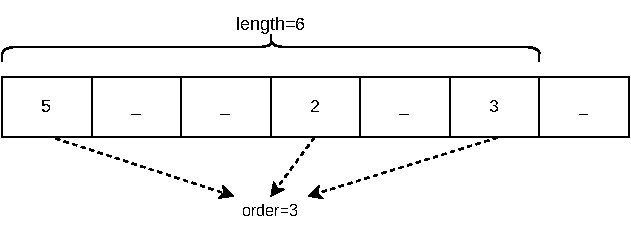
\includegraphics[width=0.7\textwidth, center]{schema}
    \caption[Example of a schema]{Example of a schema, where “don’t care” symbol marked as underscore $\_$.}
    \label{fig:schema}
\end{figure}